\section{Results}
\label{sec:results}

We report three results. First, the all-site \AvgDP{} comparison
reverses sign when the LUT baseline is replaced by a decomposed-AIG
baseline at comparable small-gate granularity. Second, target-layer
\AvgDP{} is invariant across the three representations. Third, the
ARX-versus-substitution \AvgBW{} gap is stable across the representation
controls. We close with the synthetic MAJ-$n$ experiment as a
forward-looking mechanism study.

% =============================================================================
\subsection{The AOIG-to-MIG comparison depends on granularity}
\label{sec:results:granularity}

The original LUT/AOIG-to-MIG comparison is reproducible: on the 15
circuits, all-site \AvgDP{} changes by a mean of $-13.0\%$, with
$13/15$ circuits showing lower \AvgDP{} under MIG. This number is not
wrong, but it is not stable. When the baseline is a decomposed 2-input
AIG at comparable small-gate granularity, the sign reverses: AIG$\to$MIG changes all-site \AvgDP{}
by a mean of $+21.4\%$, and no circuit shows a reduction.
Table~\ref{tab:granularity_confound} lists both comparisons.

\begin{table}[t]
\centering
\caption{All-site \AvgDP{} change (\%) from AOIG to MIG by baseline.
         Negative = MIG has lower \AvgDP{}; positive = MIG has higher.}
\label{tab:granularity_confound}
\footnotesize
\begin{tabular}{@{}lrr@{}}
\toprule
Circuit & LUT$\!\to\!$MIG & AIG$\!\to\!$MIG \\
\midrule
\multicolumn{3}{@{}l}{\textit{4-bit S-box}} \\
\quad PRESENT S-box       & $-21.5$ & $+7.6$  \\
\quad GIFT S-box          & $-16.8$ & $+8.3$  \\
\quad PRINCE S-box        & $-23.7$ & $+9.2$  \\
\quad PRINCE S-box$^{-1}$ & $-23.1$ & $+14.5$ \\
\multicolumn{3}{@{}l}{\textit{Substitution round}} \\
\quad GIFT subcells  & $-16.8$ & $+7.8$  \\
\quad GIFT round     & $-16.8$ & $+18.7$ \\
\quad PRESENT round  & $-19.8$ & $+16.7$ \\
\multicolumn{3}{@{}l}{\textit{Permutation}} \\
\quad PRINCE $M'$    & $-10.0$ & $+20.0$ \\
\multicolumn{3}{@{}l}{\textit{SIMON}} \\
\quad SIMON-32       & $-11.1$ & $+47.7$ \\
\quad SIMON-64       & $-11.1$ & $+47.7$ \\
\multicolumn{3}{@{}l}{\textit{Keccak-$\chi$}} \\
\quad 5-bit          & $+8.0$  & $+11.7$ \\
\quad 64-row         & $+8.0$  & $+11.7$ \\
\multicolumn{3}{@{}l}{\textit{ARX}} \\
\quad SpecKey        & $-13.9$ & $+38.1$ \\
\quad Speck-32       & $-12.5$ & $+24.0$ \\
\quad MARX-2         & $-13.8$ & $+37.9$ \\
\midrule
\textbf{Mean} & $\mathbf{-13.0}$ & $\mathbf{+21.4}$ \\
\bottomrule
\end{tabular}
\end{table}


\begin{figure}[tbp]
  \centering
  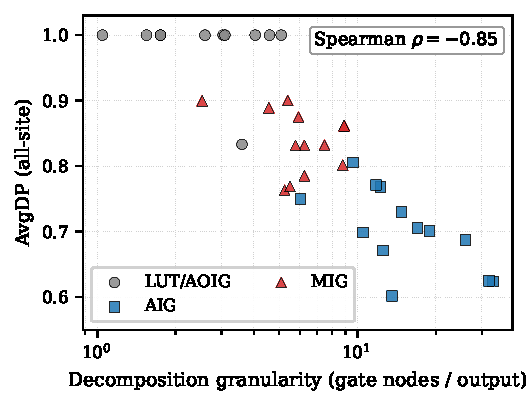
\includegraphics[width=\columnwidth]{../figures/granularity_curve}
  \caption{All-site \AvgDP{} versus decomposition granularity, measured
  as gate-output fault sites per primary output. Across LUT/AOIG, AIG,
  and MIG representations, \AvgDP{} is associated with
  representation granularity (Spearman $\rho=-0.85$ in the generated
  artifact).}
  \label{fig:granularity-curve}
\end{figure}

The mechanism is the site distribution described in
\S\ref{sec:methodology:mechanism}. A wide LUT that directly drives a
primary output contributes one output-adjacent site with high detection
probability. A decomposed-AIG or MIG contributes many interior sites, and
their effects can be masked by downstream gates. Averaging over all
sites therefore mixes a logic question with a representation-size
question. The same circuit can appear to gain or lose fault
observability depending on which baseline supplies the fault-site
population.

% =============================================================================
\subsection{Target-layer AvgDP is representation-invariant}
\label{sec:results:target-layer}

Restricting the campaign to output-driving gates removes the interior
site mix. On the evaluated circuits, target-layer \AvgDP{} is exactly
1.000 for LUT/AOIG, AIG, and MIG representations; the mean spread
across flows is 0.000. Table~\ref{tab:representation_robustness}
reports this together with the ARX/substitution \AvgBW{} ratio across
representations.

% Auto-generated by scripts/gen_reframe_tables.py
\begin{table}[t]
\centering
\caption{Granularity controls. Target-layer \AvgDP{} (output-driving gates only) is $1.000$ across all representations: the all-site difference is interior-node mix, not a changed output layer. ARX/substitution \AvgBW{} ratio is likewise stable in this benchmark, supporting an architecture-level interpretation.}
\label{tab:representation_robustness}
\begin{tabular}{lcc}
\toprule
Representation & Target-layer AvgDP & ARX/Subst.\ AvgBW \\
\midrule
LUT/AOIG & $1.000$ & $1.85\times$ \\
AIG & $1.000$ & $1.86\times$ \\
MIG & $1.000$ & $1.92\times$ \\
\bottomrule
\end{tabular}
\end{table}


This does not mean target-layer faults are the only physical faults an
attacker can induce. It means that when the target layer is held fixed,
the apparent synthesis-flow \AvgDP{} difference disappears on this
benchmark. We therefore treat all-site \AvgDP{} as a useful structural
descriptor of a netlist, but not as a representation-independent
security metric.

% =============================================================================
\subsection{ARX avalanche breadth is stable across representations}
\label{sec:results:arx}

The architecture-level \AvgBW{} result survives the granularity
controls. In the MIG flow, ARX primitives have mean \AvgBW{} $=2.056$
across Speck-32, SpecKey, and MARX-2, while the substitution-based pool
has mean \AvgBW{} $=1.082$. Every ARX value exceeds every
substitution-based value, giving a $1.90\times$ ratio
(one-sided exact Mann-Whitney $p=0.0083$). The ratio remains between
$1.85\times$ and $1.92\times$ across LUT/AOIG, AIG, and MIG
representations (Table~\ref{tab:representation_robustness}).

\begin{table}[tbp]
  \caption{Mean \AvgBW{} by cipher family (MIG flow). ARX primitives average $2.06$ output bits corrupted per detected fault versus $1.08$ for substitution-based primitives; the ratio is $1.90\times$ (Mann--Whitney $p=0.0083$). Stable across LUT/AOIG, AIG, and MIG representations (Table~\ref{tab:representation_robustness}).}
  \label{tab:arx-dichotomy}
  \centering
  \small
  \begin{tabular}{lrrcr}
    \toprule
    Family & $N$ & mean AvgBW & [min, max] & $\sigma$ \\
    \midrule
4-bit S-box & 4 & 1.013 & [1.00, 1.04] & 0.018 \\
    Subst. round & 3 & 1.173 & [1.00, 1.52] & 0.245 \\
    Permutation & 1 & 1.000 & [1.00, 1.00] & 0.000 \\
    SIMON & 2 & 1.000 & [1.00, 1.00] & 0.000 \\
    Keccak-$\chi$ & 2 & 1.000 & [1.00, 1.00] & 0.000 \\
    ARX & 3 & 2.056 & [1.71, 2.24] & 0.243 \\
    \bottomrule
  \end{tabular}
\end{table}


\begin{figure}[tbp]
  \centering
  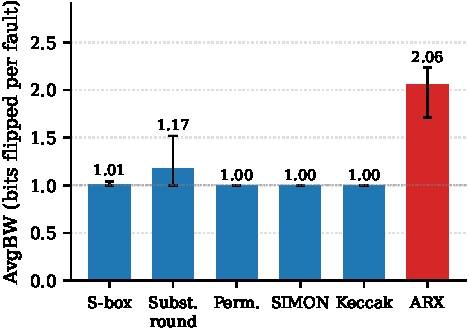
\includegraphics[width=\columnwidth]{../figures/arx_dichotomy}
  \caption{Mean \AvgBW{} by cipher architecture family in the MIG flow.
  Error bars show observed range $[\min,\max]$ over each family.}
  \label{fig:arx-dichotomy}
\end{figure}

The likely mechanism is addition-chain carry propagation: a single
internal fault in an ARX adder can change several downstream sum bits.
This is an architecture-level observation, not an exploitability claim.
Whether broader output differences help or hinder a concrete DFA depends
on the cipher's algebraic constraints and round structure.

% =============================================================================
\subsection{Higher-arity majority remains a forward path}
\label{sec:results:majn}

The granularity result tempers the interpretation of the current MIG
flow, but it does not invalidate the local masking mechanism. If a
technology provides native higher-arity majority gates, a fault entering
one input is masked whenever the remaining inputs already determine the
vote. For odd arity $n$, that masking probability is
$1-\binom{n-1}{(n-1)/2}/2^{n-1}$.

We tested direct BLIF truth-table primitives for MAJ-3, MAJ-5, and
MAJ-7 in matched synthetic chains and trees. Table~\ref{tab:majn-arity}
shows monotone \AvgDP{} reductions from MAJ-3 to MAJ-5/7, ranging from
18\% to 62\% depending on topology.

\begin{table*}[tbp]
  \caption{Synthetic MAJ-$n$ observability (chain $D{=}5$, tree $D{=}3$). \AvgDP{} drops 18--62\% from MAJ-3 to MAJ-7. $P_\text{mask}$ = theoretical per-input masking probability for odd arity $n$.}
  \label{tab:majn-arity}
  \centering
  \small
  \begin{tabular}{rrrrrrrr}
    \toprule
          &              & \multicolumn{3}{c}{Chain $D{=}5$} & \multicolumn{3}{c}{Tree $D{=}3$} \\
    \cmidrule(lr){3-5} \cmidrule(lr){6-8}
    Arity & $P_\text{mask}$ & Gates & FC\% & AvgDP & Gates & FC\% & AvgDP \\
    \midrule
3 & 0.5000 & 5 & 100.00 & 0.3875 & 13 & 100.00 & 0.3656 \\
    5 & 0.6250 & 5 & 100.00 & 0.3173 & 31 & 100.00 & 0.2057 \\
    7 & 0.6875 & 5 & 100.00 & 0.2899 & 57 & 100.00 & 0.1394 \\
    \bottomrule
  \end{tabular}
\end{table*}


This is best read as a technology hypothesis. It suggests that native MAJ-$n$
libraries could shift fault propagation if the synthesis flow preserves
MAJ-$n$ as a primitive. It does not rescue the all-site LUT-to-MIG
comparison for today's MAJ-3 decomposition flow.
